%\documentclass[review]{elsarticle}
\documentclass[]{elsarticle}
\usepackage{underscore}
\usepackage{tikz}
\usepackage{tikz-uml}
\usetikzlibrary{positioning}
\usetikzlibrary{calc}
\usetikzlibrary{shapes.misc}
\usetikzlibrary{through,arrows} % for circle of nodes ...
\usetikzlibrary{shapes.arrows, fadings}

\newif\ifsummary
\summarytrue % or \draftfalse
\summaryfalse % or \draftfalse

\newcommand*\rot{\rotatebox{90}}

\usepackage{local-tikz-style}

%% for in-line code: https://tex.stackexchange.com/questions/19004/how-to-format-an-inline-source-code
\usepackage{listings}
\usepackage{color}
\definecolor{lightgray}{gray}{0.9}
\definecolor{llgray}{gray}{0.9}

\lstset{
    showstringspaces=false,
    basicstyle=\ttfamily,
    keywords={Tier 1, Tier 2},
    %keywordstyle=\color{blue},
    keywordstyle=\ttfamily,
    commentstyle=\color[grey]{0.6},
    breaklines=true,
    stringstyle=\ttfamily
}
\newcommand{\code}[2]{\lstinline[style=Inline,language=#1]$#2$}
\newcommand{\cdx}[1]{\code{Python}{#1}}
%% end in-line extras

\usepackage{lineno,hyperref}
\modulolinenumbers[5]

\journal{Journal of \LaTeX\ Templates}

%%%%%%%%%%%%%%%%%%%%%%%
%% Elsevier bibliography styles
%%%%%%%%%%%%%%%%%%%%%%%
%% To change the style, put a % in front of the second line of the current style and
%% remove the % from the second line of the style you would like to use.
%%%%%%%%%%%%%%%%%%%%%%%

%% Numbered
%\bibliographystyle{model1-num-names}

%% Numbered without titles
%\bibliographystyle{model1a-num-names}

%% Harvard
%\bibliographystyle{model2-names.bst}\biboptions{authoryear}

%% Vancouver numbered
%\usepackage{numcompress}\bibliographystyle{model3-num-names}

%% Vancouver name/year
%\usepackage{numcompress}\bibliographystyle{model4-names}\biboptions{authoryear}

%% APA style
%\bibliographystyle{model5-names}\biboptions{authoryear}

%% AMA style
%\usepackage{numcompress}\bibliographystyle{model6-num-names}

%% `Elsevier LaTeX' style
\bibliographystyle{elsarticle-num}
%%%%%%%%%%%%%%%%%%%%%%%

\begin{document}

\begin{frontmatter}

\title{Using ISO standards to design a metadata registry for climate data}
%%\title{Elsevier \LaTeX\ template\tnoteref{mytitlenote}}
%%\tnotetext[mytitlenote]{Fully documented templates are available in the elsarticle package on \href{http://www.ctan.org/tex-archive/macros/latex/contrib/elsarticle}{CTAN}.}

%% Group authors per affiliation:
\author{Martin Juckes}
%%\author{Elsevier\fnref{myfootnote}}
\address{Rutherford Appleton Laboratory, Didcot, UK}
%%\fntext[myfootnote]{Since 1880.}

%% or include affiliations in footnotes:
%%\author[mymainaddress,mysecondaryaddress]{Elsevier Inc}
%%\ead[url]{www.elsevier.com}

%%\author[mysecondaryaddress]{Global Customer Service\corref{mycorrespondingauthor}}
%%\cortext[mycorrespondingauthor]{Corresponding author}
%%\ead{support@elsevier.com}

%%\address[mymainaddress]{1600 John F Kennedy Boulevard, Philadelphia}
%%\address[mysecondaryaddress]{360 Park Avenue South, New York}

\begin{abstract}
The climate modelling community collaborate globally to generate a coordinated portfolio of climate simulations which serve to advance scientific understanding and to support the Assessment process of IPCC. 
The interoperability of data products among the participating institutions is guaranteed by a detailed specification of the parameters to be archived and the associated metadata requirements.
This paper looks at the potential for increasing interoperability towards users outside this core community by expressing metadata requirements through the language of ISO standards on metadata registries. 
\end{abstract}

\begin{keyword}
Data registry\sep
Climate data management
\end{keyword}

\end{frontmatter}

\linenumbers



%% standards references not set well as stands ... can modify the titles or look for other styles in article-header.

%% beging document is embedded in article-header
%%\begin{document}

Lopez-Lorca, A. A., Beydoun, G., Valencia-Garcia, R., \& Martinez-
Bejar, R. (2016). Supporting agent oriented requirement analysis
with ontologies. International Journal of Human-Computer
Studies, 87(2016), 20–37.
%%
%% referenced in "Agent-based ...." as source of ontologies



Using MOF: https://link.springer.com/chapter/10.1007/978-3-319-67271-7_7 (need to buy/order).
Model Driven Architecture

\verb+http://www.geocities.ws/pravin_suman/Resources/00-11-05.pdf+

A meta-model for the analysis and design of organizations in multi-agent systems https://ieeexplore.ieee.org/abstract/document/699041,

https://www.semanticscholar.org/paper/Aalaadin\%3A-A-Meta-Model-for-the-Analysis-and-Design-Ferber-Gutknecht/db9a005b8dfdcd98482e27a6faf45c4d8fca50f2 -- appears to describe an information management system .. 

\section{Introduction}

The wide exchange of climate model output underpins a growing awareness of the severe challenges of accelerating climate change.
This paper considers one aspect of the standardisation work which is needed to ensure the timely distribution of
accessible data products: the specification of thousands of physical parameters calculated and shared from all participating
institutions. The specifications include definitions of parameters, technical metadata requirements and information on the intended use of 
the parameter.

The global policy framework for responding to the multiple threats and challenges of climate change
draws on regular assessments from the Intergovernmental Panel on Climate Change (IPCC) providing an overview of the state of knowledge, where consensus can be found\footnote{this is a significant and substantial caveat}, 
concerning the science of climate change. Projections of possible future outcomes from climate models based
on a range of different social and industrial actions provide the foundation for the assessment of the impact of future climate variability.
The climate projections come from multiple independent research institutions, in a global activity known as the
Coupled Model Intercomparison Project (CMIP).
This is an activity of World Climate Research Program (WCRP) which is overseen by the Working Group on Coupled Models (WGCM).
While the IPCC assessments are developed in a carefully designed framework agreed at an intergovernmental level, 
the climate projections being assessed are deliverd by the research community through a broad
range of independentally managed research programmes, projects and activities. Coordination is provided through two
expert panels set up by WGCM: the CMIP Panel and the WGCM Infrastructure Panel.

The public debates around climate variability focus on a handful of physical parameters, such as temperature, rainfall, and wind speeds.
The demand for thousands of physical parameters arises from the crucial need to understand the reliabilty of the climate model
output. The exchange of data serves not only to produce the headline graphs of rising temperatures, but also provides
the basis for a forensic examination of the processes represented by the models in order to assess their credibility
and guide future developments \citep[see][]{Eyring2016}. 

The scope of the physical processes covered by the climate models is rapidly expanding.
Setting the standards to encompass this scope in the context of an extensive community of independent research scientists
brings many organisational and technical challenges [[specify]].

This paper is not a formal plan for delivering services with agreement among the parties concerned: it is a provider perspective
on options for improving the accuracy and efficiency of the processes that govern the development and the maintenance 
of the relevant metadata.

The CMIP6 Data Request \citep[DREQ][]{juckes2019disc} provides detailed technical specifications of thousands of
climate parameters which are being
archived by climate modelling centres around the world as part of a global effort to update the set of reference
climate simulations which guide global policy on climate change mitigation and adaptation. 

\section{Background}\label{sec:bg}

\subsection{Exploiting the International Standards Organisation [ISO]}\label{sec:iso}

The ability to discuss the whole range of issues from governance to comprehensive technical details is a valuable 
strength of the ISO standards. This is of particular relevance in the context of a metadata registry which is
constructed through wide community engagement. Different categories of technical information require different
forms of approval and harmonisation. This paper aims to clarify the procedures, roles and responsibilities
through the ISO framework.

The main pillars of the work are the standards listed here: 

\begin{itemize}
\item QU Quantities and Units: Parts 1: General \cite{iso80000-1},
         3: Space and Time \cite{iso80000-3}, 4: Mechanics \cite{iso80000-4}, 5: Thermodynamics \cite{iso80000-5},
         7: Light and Radiation \cite{iso80000-7}, and  9: Physical Chemistry and Molecular Physics \cite{iso80000-9}.
%%\item QU-ST Quantities and Units (80000-3 {Space and Time})
%%\item QU-ME Quantities and Units (80000-4 {Mechanics})
%%\item QU-TH Quantities and Units (80000-5 {Thermodynamics})
%%\item QU-AC Quantities and Units (80000-7 {Light and Radiation})
%%\item QU-NP Quantities and Units (80000-9 {Physical Chemistry and Molecular Physics})
\item GIM Geographic Information --- Metadata (19115-1 \cite{iso19115-1})
\item GIP Geographic Information --- Procedures (19135-1 \cite{iso19135-1})
\item MDR Metadata Registries (11179)
\item ITG Governance of Information Technology \cite{iso38500}
\item EIF Enterprise integration — Framework for enterprise modelling, \cite{iso19439} 
\item EIC Enterprise integration — Constructs for enterprise modelling, \cite{iso19440}
\item MOF OMG Meta Object Facility \cite{iso19508}
\item GPD General Purpose Datatypes \cite{iso11404}
\end{itemize}

All these standards can contribute, but the primary focus here will be on the interplay between structures of the metadata registry
and the organisations around it as seen through the language of MDR and EIC. MOF will be used as an organisational structure.

These three standards are all about standardising modeling approaches for describing implementations (or descibing modelling processes in the case
of MOF) rather than standardised implementations.


\begin{figure}[h]
\begin{tikzpicture}
\umlsimpleclass[sc1,y=0,type={mdr}]{Registry}
\umlsimpleclass[sc1,y=-3,x=9,type={EIC}]{Organisation}
\umlsimpleclass[sc1,y=-3,x=0,type={mdr}]{Register}

\umlcompo[link1,arg2={Functional Entity},align2=left,pos2=0.95,stereo={resource}, anchor stereo=west]{Organisation}{Registry}
\umlcompo[link1,arg2={Organisational Element}, mult2=*]{Registry}{Register}
\umldep[link1, % arg1=mdr, arg2=eic,
            stereo={abstraction}]{Register}{Organisation}
\end{tikzpicture}
\caption{Top level relationship between Registry and Organisation. In a sense the Registry contains the Organisation as a modeled concept and the Organisation contains the Registry as a defined function. More precisely, the Registry contains an abstraction of the Organisation.}
\label{fig:mdr-eic}
\end{figure}

\cite{sinaci2013} describes the use of ISO 11179 to facilitate exchange across clinical work and care domains.
5 odp viewpoints

 The approach used here resembles that described by McClatchey\cite{mcclatchkey2018}: a layered approach is used, and objects in
the model are described as registered items.
The resulting model is used to implement
a systematic approach to collecting provenance information in a distributed
software system.
Here we are looking at a somewhat different problem of capturing provenance information arising from multiple interacting science teams and institutions.
From a modeling perspective, there is some similarity.
Setting out the requirements for provenance collection clearly in the upper layers of the m-cake provides a systematic framework for embedding the functionality consistently in a range of different artefacts at the workflow implementation layer. 

\subsection{Meta Object Facility (MOF)}\label{sec:mof}

The Meta Object Facility\cite{iso19508} (MOF) of the Object Modeling Group (OMG) formalises the process of developing a conceptual
outline into a functioning system into discrete steps and
defines a modeling language to express the procedures for moving the design up to the next level.
It is a model-based approach, so that the definition of the modeling language preceeds, in the MOF-sequence, the
definition of key organisational or functional units. In practise, we are building many parts of the model around
pre-existing structures, so that the model serves as a formalised representation of an existing system rather than a design specification. 

The first stage of implementing MOF is define the number and purpose of the MOF layers. A four layer approach is commonly used, 
though this is not obligatory. Within the four layer approach, there are different characterisations of the layers for
different kinds of modeling. In engineering, for instance, the lowest level may refer to physical objects which have been created, such as
the four layer model described in the review by Djuric et al.\cite{djuric2006}:
``Real World'', ``Model'', ``Meta-model'', ``Meta-meta-model''.
%http://www.jot.fm/issues/issue_2006_11/article4/article4.pdf
In a variation on this theme, Inan et al.\cite{inan2018} model a disaster response system which brings some of the people,
called ``agents'' in this context, into the model.
They follow the above terminology, referring to the M0 layer as ``Real World'' and M1 as ``Model'', but, in an interesting twist,
their MOF implementation places
a number of active agents playing managerial and coordination roles in the ``Model'' layer.
The M0 layer consists of elements which are engaging directly with the physical aspects of disaster response.
%http://www.jot.fm/issues/issue_2006_11/article4/article4.pdf

In the software engineering domain, on the other hand, the lowest level is usually described as the application layer.
The following four layers:
``Application'', ``Semantic'', ``Object'', ``Syntax'' have been proposed for information modelling on the web\cite{melnik2000}. 
%%[http://infolab.stanford.edu/~melnik/pub/sw00/]
%% A Layered Approach to Information Modeling and Interoperability on the Web 2000-30.pdf

\subsubsection{MOF Layers and Enterprise Integration Phases}

Here we wish to describe database with associated software, and also the surrounding organisation and interactions which contribute
content to the database.
In order to get full provenance information, it is important to represent the agents responsible for
the creation of metadata elements, and hence we wish to include the agents in the model and will follow this aspect of Inan et al.
by representing active agents in the M1 layer, and even in the M2 layer. In order to avoid the unfortunate connotation
that these are in some way un-real, we introduce new terminology for the layers:
``Delivery'' -- ``Design'' -- ``Definition'' -- ``Domain''.

The EIF specifies seven model phases in the specification of an organisation:
domain identification, concept definition, requirements definition, design specification, implementation description, domain operation, and decommission definition.
There are also three levels of genericity: "generic", "partial" and "particular".  The these levels allow progressive
increase in the level of detail provided. 

In order to exploit EIF within the MOF framework, we align the MOF layers with the EIF model phases:
\begin{itemize}
\item M3 Domain: domain identification;
\item M2 Definition: concept definition, requirements definition;
\item M1 Design: design specification, implementation description;
\item M0 Delivery: domain operation, and decommission definition.
\end{itemize}


The use of Factory elements to represent implementation rules allow the model to be responsive, rather than prescriptive. That is, the implementation decisions are taken by the agents working within the design and implementation elements of the model.
This allows the model to represent community groups which are critical to the process of establishing standards without prescribing 
structures which constrain them. The model does prescribe some requirements to enable transparency of decision making.


\begin{table*}[tb]
        \centering
        \caption{MOF}
        \label{tab:mof}
        \begin{tabular}{|c|l|p{5cm}|p{5cm}|}
\hline
3 & Concept & \multicolumn{2}{c}{MOF Profile, Layers, Modelling languages} \cr
\hline
2 & Requirements & Configuration Schema, Base Classes, Package Outlines, Profile of MDR &  Profile of EIC \cr
\hline
1 & Design & Registry Schema, Configuration, Sample, Python Classes & Organisational Elements, Decision Points, Specifications of Roles \cr
\hline
0 & Delivery & & \cr
\hline
\end{tabular}
\end{table*}


\subsubsection{Domain identification using EIC}

{\color{red} MOVE:: 
The objective is to construct executable models, but the concept of ``execution'' is broad enough to include the usage of ``executing a project''.
The apex layer of the MOF stack should describe the four layers.}


EIC specifies that domain identification should include specification of "inputs and outputs and their respective origins and destinations", and specifies a set of constructs which are needed to adequately identify the domain.

\begin{table*}[tb]
        \centering
        \caption{Domain identification}
        \label{tab:domi}
        \begin{tabular}{|p{3cm}|p{9cm}|}
Name  & Climate Science Metadata Registry \cr
Design Authority &  \cr
Description & \cr
Business Process Description & \cr
Objectives & Strategic:  \cr
Constraints & Availability of staff resources; community engagement; \cr
Object View Inputs &   DM-X Project       OV-1 Data  \cr
Event Inputs & \cr
Object View Outputs & \cr
Event Outputs & \cr
\end{tabular}
\end{table*}

% 6.3
BP Business Process -- describes functionalities, desired results, and objectives. Attached to OV and Enterprise Activity at requirements definition phase an OU at the design specification phase.

% 6.10
RE Resource -- Capabilities of tools, devices, etc (not people). Named at the identify phase, details added at design specification, including links to Operational Role and Capability.

% 6.6
EO Enterprise Object -- describing a persistent entity in the organization being modeled: e.g. person, order, file.
PR Product -- describes a product. Linked to EO and (at design phase) OU and OR

% 6.9
OR Order -- an instruction for performance of an operation. Links to EO and (at design specification phase) OU.

% 6.17.4
%%OPR Operational Role -- describes the skill profile needed for undertake defined operational tasks. Job description added at the requirements definition phase.
% 6.13
OU Organizational Unit -- a component in the organizational structure of the modeled entity. E.g. department, section, group. Can have EO assets and an Organizational Role

EV Event

OV Object View -- List attributes of an EO needed for a specific purpose.
%% see fig D.11

\begin{figure}[h]
\begin{tikzpicture}
%% perhaps want a longer title here ... of just make this the "SKOS:techLabel" -- map EIC attributes to SKOS ...

\coordinate (ofv) at (7.5,0.5);
\coordinate (orv) at (5.5,-3.5);

%%\draw[white,fill=black!5] (0.,1.5) rectangle (12.,-4.5);% Function
%%\draw[orange,fill=orange!30] (ofv) rectangle (12.,-3.5);% Function
%%\draw[orange,fill=blue!30]   (orv) rectangle (12.,-6.5);% Resource
%%\draw[orange,fill=red!10]   (0.,-4.0) rectangle (5.,-6.5);% Organisation

\umlsimpleclass[sc1,x=5,y=2,type={Domain}]{Registry Service}

\umlsimpleclass[func,y=+0.1,x=7.8,type={BP}]{Standards}
\umlsimpleclass[func,y=-1.1,x=8.2,type={BP}]{Registration}
\umlsimpleclass[func,y=-2.3,x=8.6,type={BP}]{Management}
\umlsimpleclass[func,y=-3.5,x=8.6,type={BP}]{Activity}

%%\umlsimpleclass[inf,y=-2.5,x=4,type={EO}]{Person}
\umlsimpleclass[inf,y=1.,x=8,type={EO}]{Document}


\umlsimpleclass[inf,y=1.,x=0,type={EO}]{Project}
%%%\umlsimpleclass[inf,y=1.,x=4,type={EO}]{infrastruc}

\umlsimpleclass[inf,y=-0.5,x=0.5,type={OR}]{Order}
\umlsimpleclass[inf,y=0.5,x=4,type={EV}]{Agreement}

\umlsimpleclass[inf,y=-2.8,x=4,type={EO}]{Software}
\umlsimpleclass[inf,y=-2.,x=0.5,type={EO}]{Registry Item}

\umlsimpleclass[resrc,y=-5.3,x=4.5,type={EO}]{Platform}


%%\umlsimpleclass[resrc,y=-6,x=8,type={Role}]{Staff} %% added at later model stage ...
\umlsimpleclass[resrc,y=-4.3,x=8,type={Resource}]{Service}
\umlsimpleclass[resrc,y=-5.3,x=8,type={Resource}]{Environment}

%%
%% these don't really belong here .....
%% wrong category of thing ..
%%\umlsimpleclass[inf,y=-4,x=1,type={EV}]{Event}  
%%\umlsimpleclass[inf,y=-2,x=1,type={OV}]{Object View}

\umlsimpleclass[org,y=-3.3,type={OU}, width=7cm]{Community}
\umlsimpleclass[org,y=-4.5,type={OU}, width=7cm]{Information Technology}
\umlsimpleclass[org,y=-5.7,x=1,type={OU}, width=7cm]{Communications}

%%\umlnote[note1, y=-6.cm, x=9cm, width=7cm]{Environment}{Linked to Operational Role and Capability descriptions at
%% the design specification phase}


\umlassoc[link1,geometry=|-,arg1=implements]{Agreement}{Standards}
\umlassoc[link1,geometry=-|-,arg1=creates]{Registry Item}{Registration}
%%\umlcompo[link1]{Registry Service}{Standards}
%%\umlcompo[link1]{Registry Service}{Management}
%%\umldep[link1, % arg1=mdr, arg2=eic, stereo={abstraction}]{Register}{Organisation}
\end{tikzpicture}
\caption{Domain identification, generic level. At this level, the Event, Order and Object View classes are modified
only through the specification that they are sub-classes of the MDR base class. Other classes are named and given descriptons listed in section [[SSS]]. Following figure B.2 of EIF. [[IN TEXT??]] In software systems the distinction between an object and a resource can become blurred: it is natural to treat virtual machines like machines ... but here we stick with the standard and assign ... ; here the resource is }
\label{fig:domident}
\end{figure}

% Annex E of EIC lists typical usage of these at the different phases.
At the M2 level we add Decision Centre, Enterprise Activity, Capability, Organizational Role, Operational Role and
Decision Centre. 

The Enterprise Activity captures time-limited activities, such as creating a registered item or running a service for 12 months. EA is employed by a single Business Process and is delivered by an Operational Role. 

Organizational Roles, attached to Organisational Units, contain Decision Centres.:w

Decision centre links the functional view and the 


%% for implementation, see opmsg2011 .... in particular, also examples of Event etc in EIC .
%% the completed template defines a class object.
%% SC5_N1111_OPM_SG_Interim_Report_May_2011.pdf

The \cd{EIC::concept_definition} phase includes a short textual specification of the \cd{EIC::domain} 
strategies, policies, operational concepts, and business plans. These are given given in section XXX below. In addition,"Decision Functions" should be specified.



The Delivery layer includes the organisational structures making decisions about the final products in
the metadata registry, which are the registered metadata items describing environmental quantities.


\subsection{Decision Functions}

The \cd{EIC::Decision_Function} concepts define a set of related decisional activities. The three categories of decisions needed here relate to:
%% registration and management? 
\begin{itemize}
\item \cd{Parameter Registration}
\item \cd{Standard Registration}
\item \cd{Standard Registration}
\end{itemize}

\subsection{Reflection}

In the object modeling community, ``reflection'' refers to the ability of an object to contain a description of itself. For an example, a library may be reflective if it contains a book describing the construction and maintenance of the building and its contents. 

We follow MOF in creating a naming scheme for model elements, and this naming scheme will be used to embed the model
in the metadata registry which is to be implemented as the final stage of the work.

We adopt the common notation of a double-colon for scope resolution and a period for attached entities. Thus \cd{OBJECT::DESCENDANT} refers to an entity within the scope of \cd{OBJECT}, and this scope is interpreted as consisting of all entities which are instantiated from \cd{OBJECT} or [[associations?]].

\cd{OBJECT.CHILD} refers to an attribute or method which is defined to be part of \cd{OBJECT}.

[[ is it necessary to create a container for ``universal'' attributes, so that there is no conflict, e.g. \cd{OBJECT.__global__.parent}? Is double underscore allowed?

The reflective elements of an \cd{OBJECT} will be given by a ``parent'' and an ``origin''. The ``parent'' is the classifier and the ``origin''
is the context in which the classification took place, which should be an instance of a MOF Factory. Generally, the creation of an object
requires that configuration information be added to the parent. The ``origin'' object should provide information around this process.


\verb+ ID  = "DRM" :: PACKAGE [ ATTRIBUTE | | :: CLASS [ ATTRIBUTE | ] ] +

E.g. \verb+DRM::register.var.tas::title = \+

\subsection{Factories, Orchestration, Stereotypes and Provenance}

Management of provenance information is a critical part of the devlopment and maintenance of standards.
This is a significant challenge here because the development work can involve staff from hundreds of institutions
working in ad-hoc teams.

The EIC organisation structure defines decision centres and functions. Instantiation is a specific category of functional operation.
In EIC the functional operation is performed within and \cd{EIC_Enterprise_Activity} using a \cd{EIC_Functional_Entity} (which is a type of resource). The specification of the \cd{EIC_Functional_Entity} identifies the inputs and outputs of the functional operation.


The category of 


\begin{figure}[h]
\begin{tikzpicture}
\umlsimpleclass[sc1,y=0,type={collection}]{IconicBuildings}
\umlsimpleclass[sc1,y=0,x=8,type={instance}]{EmpireState}
\umlsimpleclass[sc1,y=-3,x=0,type={design}]{Quantity}
\umlsimpleclass[sc1,y=-3,x=8,type={instance}]{Air Temperature}
\umlsimpleclass[sc1,y=-6,x=0,type={require}]{Work Group}
\umlsimpleclass[sc1,y=-6,x=8,type={instance}]{Harmonisation Team}

\umlinherit[link1,stereo={admit}]{EmpireState}{IconicBuildings}
\umlinherit[link1,stereo={create}]{Air Temperature}{Quantity}
\umlinherit[link1,stereo={co-develop}]{Harmonisation Team}{Work Group}
%%\umlcompo[link1,arg2={Organisational Element}, mult2=*]{Registry}{Register}
%%\umldep[link1, % arg1=mdr, arg2=eic,
            stereo={abstraction}]{Register}{Organisation}
\end{tikzpicture}
\caption{Different aspects of specialisation.}
\label{fig:mof-inst}
\end{figure}

\section{More about the data request}

The DREQ is part of a range of infrastructure projects \citep{Balaji2018}. See also ES-DOC \citep{pascoe2019disc}.

The current practise is that the delivery layer includes, in effect, a model in a domain specific syntax. That is, the specifications
for a data variable can be considered as defining a UML class which is instantiated to create data files.

In the language of this study, the factory which orchestrates the instantiation of data specifications into files ready for archive
is beyond the scope of this paper. 

The general scope of the different layers has been introduced in DREQ, where M2-0 are described as the  
framework, configuration and content respectively.
The more formal approach described here introduces a clearer
demarkation of the layers and enables a structured extension to encompass an improved 
representation of the organisational structures which surround the technical components of the metadata registry.


The DREQ is built on domain standards which have evolved with the CMIP project. In this paper we explore the
feasibility and potential benefits associated with expressing these specifications through ISO standards. 

The work cuts across a range of standards which are introduced in Section \ref{sec:iso} below, covering aspects of geospatial referencing, physical quantities, and the organisation and processes inherent in running a registry of metadata specifications. 

The expected benefits will be both in terms of inter-operability with other standards which deal with environmental information and also in terms of learning from and exploiting practises which are embedded in the ISO standards. 

We look at three principle areas of the activity.

Firstly, the description the overall orangisational structure. 

Secondly, community interaction which involves a broad and rapidly growing network,
with participants from hundreds of institutions and dozens of countries. The structure has evolved organically, always pressured by the rapid 
expansion of the global climate modelling activity and the societal pressures associated with growing awareness of the
risks posed by anthropogenic climate change. One of the consequences of the broad and loosely
coordinated collaboration is that names of some contributors are only recorded in email chains or online discussion.

Finally, the Information Technology.
The DREQ includes thousands of different quantities, 
all of which are defined in and registered in the CF Convention. In order to increase interoperability with
other communities this paper develops a mapping from the terms in the data request to ISO standard quantities.
We we also consider the definition of data types, including specification
of multi-dimensional arrays which combine geospatial coordinates with additional domain specific dimensions.

\begin{figure}[h]
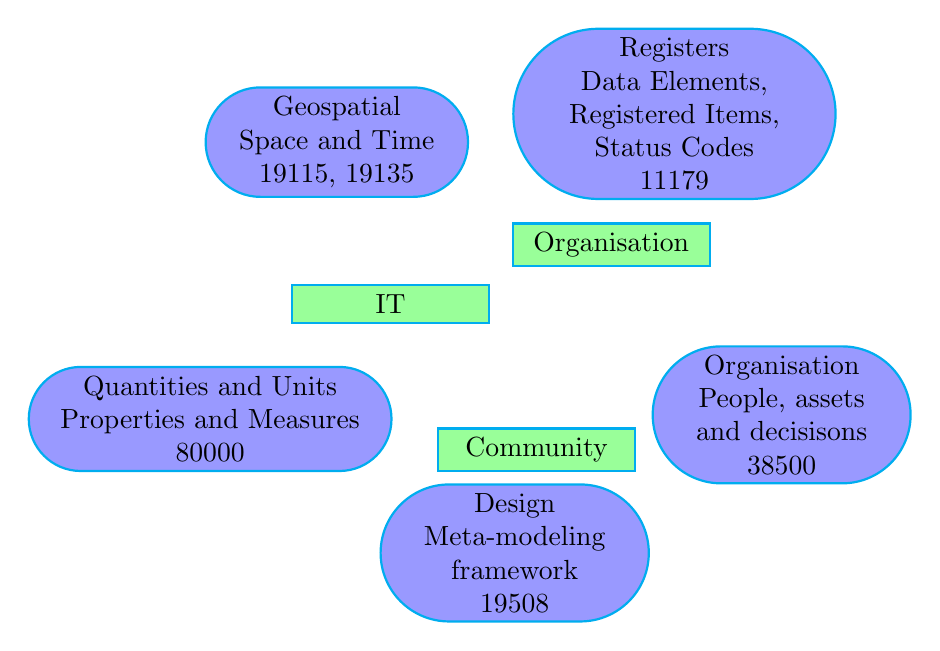
\begin{tikzpicture}[
  thick,
  every pin edge/.style={<-},
  >=latex,
  declare function/.list={
    outerR=2.0;,
    innerR=1.6;,
    angleofNode(\a)=\a/5*360-90;},
  std/.style={rounded rectangle, align=center, fill=blue!40, draw=cyan},
  chpt/.style={rectangle, minimum width=2.5cm, align=center, fill=green!40, draw=cyan}
  ]

\node [circle through=(0:outerR)] (c) {};
\node [circle through=(0:innerR)] (d) {};

%%\node[draw,chpt,anchor=90] at (d.40) {Organisation};
%%\node[draw,chpt,anchor=210] at (d.160) {IT};
%%\node[draw,chpt,anchor=330] at (d.270) {Community};
\node[draw,chpt] at (d.40) {Organisation};
\node[draw,chpt] at (d.170) {IT};
\node[draw,chpt] at (d.280) {Community};

\node[draw,std,anchor=angleofNode(2.5)] at (c.{angleofNode(0)}) {Design\\Meta-modeling\\framework\\19508};
\node[draw,std,anchor=angleofNode(3.5)] at (c.{angleofNode(1)}) {Organisation\\People, assets\\and decisisons\\38500};
\node[draw,std,anchor=angleofNode(4.5)] at (c.{angleofNode(2)}) {Registers\\Data Elements,\\Registered Items,\\Status Codes\\11179};
\node[draw,std,anchor=angleofNode(0.8)] at (c.{angleofNode(3)}) {Geospatial\\Space and Time\\19115, 19135};
\node[draw,std,anchor=angleofNode(1.5)] at (c.{angleofNode(4)}) {Quantities and Units\\Properties and Measures\\80000};

\end{tikzpicture}
\caption{The five core standards explored in this paper. The scope of these five standards overlaps in many areas, but
there do not appear to be any inconsistencies in the application discussed here.}
\label{fig:pentad}
\end{figure}


\subsection{Framing the issues}

A requested variable might be the monthly mean near-surface temperature, evaluated on a global grid for every month through the duration of a simulation. This parameter is defined by a title, a description, specification of units of measure, but also by technical data specifying that the quantity is represents air temperature at about 2m above the ground, information about which numerical experiments are to be measured (almost all for this variable, but other variables are only archived from a small selection of experiments). In all, there are over a hundred technical attributes used to define a variable.

In this paper we are not concerned with the definitions of the physical parameters, or even with the definitions of the attributes, but with the systems used to maintain and curate those definitions.

The definitions of these attributes have evolved over several cycles of CMIP. Many of the definitions are clear and well understood, but there are ambiguities and many areas of ongoing discussion regarding the best approach to dealing with new requirements which derive from the ever expanding physical complexity of the climate models and the following analysis. 

\section{Requirements}

\subsection{Areas of the Registry Model}

The registry model should be split into 3 areas, each area identified by a class instance with title and descriptions given
in the following 3 subsections.

\subsection{The Metadata Registry}

The metadata registry area of the model describes the structure of the metadate registry itself, conforming to the MDR standard.

\section{Roles, Activities and Packages}

\documentclass[tikz,border=10pt]{article}
\usepackage{tikz-uml}
\usetikzlibrary{positioning}
\usetikzlibrary{calc}

\tikzset{
  pck/.style = {
    minimum width = 3cm,
    node distance=2in,
    },
  note/.style = {
    width = 6cm,
    }
  }


\tikzstyle{empty}=[]
\tikzstyle{stereotype highlight}=[rounded rectangle, fill=green, opacity=.2, text opacity=1]
\tikzstyle{stereotype highlight cyan}=[rounded rectangle, fill=cyan, opacity=.2, text opacity=1]
\tikzstyle{stereotype highlight orange}=[rounded rectangle, fill=orange, opacity=.2, text opacity=1]

\begin{document}

\begin{tikzpicture}

\begin{umlsystem}[x=4, fill=red!10]{The data request registry}
\umlusecase [empty,x=-4.0cm,y=0cm,fill=,draw=,opacity=0] {}
\umlusecase [y=0.5cm, name=AA] {Registry}
\umlusecase [x=-0.5cm,y=-1.5cm, name=A, width=2cm] {Register Collection}
\umlusecase [x=-0.5cm,y=-3.5cm, name=B] {Register}
\umlusecase [x=-0.5cm,y=-5.5cm, name=ri, width=2cm] {Registered Item}
\umlusecase [x=3cm,y=-0.5cm, name=ryspec] {Register Framework}
\umlusecase [x=3cm,y=-2.5cm, name=regspec] {Register Specs}
\umlusecase [x=3cm,y=-4.5cm, name=rispec] {Item Specs}

\umlactor[x=-3.1cm, y=0.5cm]{registrar}
\umlactor[x=-3.1cm, y=1cm]{oversight}
\umlactor[x=-3.1cm, y=-1.5cm]{chief editor}
\umlactor[x=-3.1cm, y=-3.5cm]{wg}
\umlactor[x=-3.1cm, y=-5.5cm]{editor}
\end{umlsystem}

%% not getting definition done ...
\umldep[stereo style=stereotype highlight cyan, anchor stereo=east, pos stereo=0.25]{AA}{A}
\umldep[stereo style=stereotype highlight cyan, anchor stereo=east, pos stereo=0.25]{A}{B}
\umldep[stereo style=stereotype highlight cyan, anchor stereo=east, pos stereo=0.25]{B}{ri}
\umldep[stereo style=stereotype highlight cyan, anchor stereo=west, pos stereo=0.25]{AA}{ryspec}
\umldep[stereo style=stereotype highlight cyan, anchor stereo=west, pos stereo=0.25]{A}{regspec}
\umldep[stereo style=stereotype highlight cyan, anchor stereo=west, pos stereo=0.25]{B}{rispec}

\umlactor[x=11.2cm,y=0.5cm]{programme}
\umlactor[x=11.2cm,y=-1cm]{advisory}
\umlactor[x=11.2cm,y=-3.3cm]{devel}
\umlactor[x=11.2cm,y=-4.5cm]{specialist}
\umlactor[x=11.2cm,y=-6cm]{user}

%% would be nice to place stereotype above line ... probably need to change anchor .... occurs dozens of times in style file
%% should be straight mapping of code used for "stereo pos"
%% can use arg1, arg2, mult1, mult2 for additional info, but quickly becomes crowded
%%

\umlassoc[stereo style=stereotype highlight, draw=black!50, very thick, arg1=operate,stereo=own]{registrar}{AA}
\umlassoc[stereo style=stereotype highlight, arg1=govern,stereo=coordinate]{chief editor}{A}
\umlassoc[stereo style=stereotype highlight, arg1=define,stereo=ipr]{editor}{ri}
\umlassoc[stereo style=stereotype highlight, arg1=steward, stereo=review]{wg}{B}

\umlassoc[stereo style=stereotype highlight, stereo=exploit]{devel}{regspec}
\umlassoc[stereo style=stereotype highlight, stereo=exploit]{devel}{rispec}
\umlassoc[stereo style=stereotype highlight, stereo=exploit]{user}{ri}

\umlimpl[stereo style=stereotype highlight orange]{rispec}{ri}
\umlimpl[stereo style=stereotype highlight orange]{regspec}{B}
\umlimpl[stereo style=stereotype highlight orange]{regspec}{rispec}
\umlimpl[stereo style=stereotype highlight orange]{ryspec}{regspec}


\end{tikzpicture}

\newcommand{\cd}[1]{ {\it #1} }%

The \cd{registrar} is responisble for the operation of the \cd{registry}. 
The \cd{registry} can host multiple register collections,
consisting of a group of related \cd{registers} supporting a common user community.
Each 

\end{document}



\subsection{Technical and Organisational Structures}

The ISO 38500 standard on governance is designed to deal with corporate governance structures, but achieves its purpose through 
a high degree of flexibility. The ability to define cascading chains of responsibility, with the option, at each stage, for 
organisational units to define their own internal governance structures, makes it suitable for the highly non-corporate 
structure that assembles the CMIP Data Request.

What 38500 does specify is key concepts of an organisational system (decision centres, assets, competencies etc) and
a framework for describing them and their connections. In this implementation, these organisational classes will inherit
the basic aspects governing status etc from the 11179 apex concept.

In addition, the generalization with \cd{administer} stereotype
will be used to generate a suite of 

\subsubsection{stereotypes}

\cd{identify} adds attribute identifier referencing a \cd{MDR_Scoped_Identifier} [MDR, part 3, chapter 7, figure 5] instance.

Specialisations: require one \cd{MDR_Scoped_Identifier} in the registry namespace. 

\cd{register} adds \cd{MDR_submission_record}. A registered item may also be a designatable item.

\subsubsection{Principles of the technical schema}

Technical specifications are sometimes split between a "schema" and "vocabularies", with vocabularies containing extensible lists of
terms relevant to a specific domain or technical application. The vocabularies may be structured according to schema, and the "schema" may contain lists, so the distinction is somewhat arbitrary. 

Here, the distinction will be betweem register with MDR designated items and one with MDR registered items.

\subsection{Actors and Registers}

\subsection{Decisions and Data Elements}


\ifsummary
 %% [additional content omitted]
\else
\section{Overview of the metadata structures}


MDR defines physical quantities in terms of \cd{MDR_Object}, \cd{MDR_Property} and \cd{MDR_Processing}.
If we are describing a red car, for instance, "car" is the object and "red (color)" the property. The split 
between Object and Property in complex systems is less obvious.  

For instance, we have \cd{atmosphere_mass_content_of_convective_cloud_condensed_water}. This refers to the mass of liquid water and ice in the convective clouds, integrated vertically through an column in the atmosphere. Here, "cloud" could be considered as a proprty of the atmosphere, or it might be considered as the "object" of the measurment. The CF Convention takes a pragmatic approach to dealing with this, and constructs terms based on community usage and expert assessment of the clarity of the resulting name rather than any fixed grammatical rules. 

\begin{table*}[tb]
        \centering
        \caption{Quantities: there are 24 quantitites defined by ISO which can be conmsidered as generalizations of data request parameters. A substantial portion of the request is not covered by existing ISO quantities from 80000 and 19115:
for these parameters new quantities can be specified using 11179. Respecting the granularity and approach of the quantities listed, a further 30 new quantities are proposed. 
} 
        \label{tab:domi}
        \begin{tabular}{|p{2cm}|p{7cm}|l|}
Name  & Quantity & Units \cr
19115	& DateTime  & \cr
19115	& Angle  & \cr
19115	& Scale  & \cr
19115	& Distance  & \cr
19115	& Speed  & \cr
19115	& Area  & \cr
19115	& Volume  & \cr
19115	& Weight  & \cr
80000-3	 & 3-9.1: acceleration & \cr
80000-3	 & 3-7: time, duration & \cr
80000-4  & 4-15.1: Pressure & \cr
80000-4	 & 4-5: surface density & \cr
80000-4	 & 4-2: mass density & \cr
80000-4	 & 4-24: kinematic viscosity & \cr
80000-4	 & 4-29: mass flow rate & \cr
80000-5	 & 5-1: thermodynamic temperature & \cr
80000-5	 & 5.2: Celsius temperature & \cr
80000-5	 & 5-7: heat flow rate & \cr
80000-5	 & 5-8: areic heat flow rate/density of heat flow rate & \cr
80000-5	 & 5-33: Dew-point termperature & \cr
80000-7	 & 7-25.1: linear attentuation coefficent & \cr
80000-9	 & 9-12: mass fraction of substance B  & \cr
80000-9	 & 9-13: amount-of-substance fraction of substance B  & \cr
80000-9	 & 9-15: volume fraction of substance B  & \cr
\end{tabular}
\end{table*}

{\color{red} need to check wet-bulb and dewpoint}


\subsection{Activities and Roles}\label{sec:roles}

\verb+\documentclass[tikz,border=10pt]{article}
\usepackage{tikz-uml}
\usetikzlibrary{positioning}
\usetikzlibrary{calc}

\tikzset{
  pck/.style = {
    minimum width = 3cm,
    node distance=2in,
    },
  note/.style = {
    width = 6cm,
    }
  }


\tikzstyle{empty}=[]
\tikzstyle{stereotype highlight}=[rounded rectangle, fill=green, opacity=.2, text opacity=1]
\tikzstyle{stereotype highlight cyan}=[rounded rectangle, fill=cyan, opacity=.2, text opacity=1]
\tikzstyle{stereotype highlight orange}=[rounded rectangle, fill=orange, opacity=.2, text opacity=1]

\begin{document}

\begin{tikzpicture}

\begin{umlsystem}[x=4, fill=red!10]{The data request registry}
\umlusecase [empty,x=-4.0cm,y=0cm,fill=,draw=,opacity=0] {}
\umlusecase [y=0.5cm, name=AA] {Registry}
\umlusecase [x=-0.5cm,y=-1.5cm, name=A, width=2cm] {Register Collection}
\umlusecase [x=-0.5cm,y=-3.5cm, name=B] {Register}
\umlusecase [x=-0.5cm,y=-5.5cm, name=ri, width=2cm] {Registered Item}
\umlusecase [x=3cm,y=-0.5cm, name=ryspec] {Register Framework}
\umlusecase [x=3cm,y=-2.5cm, name=regspec] {Register Specs}
\umlusecase [x=3cm,y=-4.5cm, name=rispec] {Item Specs}

\umlactor[x=-3.1cm, y=0.5cm]{registrar}
\umlactor[x=-3.1cm, y=1cm]{oversight}
\umlactor[x=-3.1cm, y=-1.5cm]{chief editor}
\umlactor[x=-3.1cm, y=-3.5cm]{wg}
\umlactor[x=-3.1cm, y=-5.5cm]{editor}
\end{umlsystem}

%% not getting definition done ...
\umldep[stereo style=stereotype highlight cyan, anchor stereo=east, pos stereo=0.25]{AA}{A}
\umldep[stereo style=stereotype highlight cyan, anchor stereo=east, pos stereo=0.25]{A}{B}
\umldep[stereo style=stereotype highlight cyan, anchor stereo=east, pos stereo=0.25]{B}{ri}
\umldep[stereo style=stereotype highlight cyan, anchor stereo=west, pos stereo=0.25]{AA}{ryspec}
\umldep[stereo style=stereotype highlight cyan, anchor stereo=west, pos stereo=0.25]{A}{regspec}
\umldep[stereo style=stereotype highlight cyan, anchor stereo=west, pos stereo=0.25]{B}{rispec}

\umlactor[x=11.2cm,y=0.5cm]{programme}
\umlactor[x=11.2cm,y=-1cm]{advisory}
\umlactor[x=11.2cm,y=-3.3cm]{devel}
\umlactor[x=11.2cm,y=-4.5cm]{specialist}
\umlactor[x=11.2cm,y=-6cm]{user}

%% would be nice to place stereotype above line ... probably need to change anchor .... occurs dozens of times in style file
%% should be straight mapping of code used for "stereo pos"
%% can use arg1, arg2, mult1, mult2 for additional info, but quickly becomes crowded
%%

\umlassoc[stereo style=stereotype highlight, draw=black!50, very thick, arg1=operate,stereo=own]{registrar}{AA}
\umlassoc[stereo style=stereotype highlight, arg1=govern,stereo=coordinate]{chief editor}{A}
\umlassoc[stereo style=stereotype highlight, arg1=define,stereo=ipr]{editor}{ri}
\umlassoc[stereo style=stereotype highlight, arg1=steward, stereo=review]{wg}{B}

\umlassoc[stereo style=stereotype highlight, stereo=exploit]{devel}{regspec}
\umlassoc[stereo style=stereotype highlight, stereo=exploit]{devel}{rispec}
\umlassoc[stereo style=stereotype highlight, stereo=exploit]{user}{ri}

\umlimpl[stereo style=stereotype highlight orange]{rispec}{ri}
\umlimpl[stereo style=stereotype highlight orange]{regspec}{B}
\umlimpl[stereo style=stereotype highlight orange]{regspec}{rispec}
\umlimpl[stereo style=stereotype highlight orange]{ryspec}{regspec}


\end{tikzpicture}

\newcommand{\cd}[1]{ {\it #1} }%

The \cd{registrar} is responisble for the operation of the \cd{registry}. 
The \cd{registry} can host multiple register collections,
consisting of a group of related \cd{registers} supporting a common user community.
Each 

\end{document}

+

\subsection{Metadata Packages}\label{sec:packages}




\begin{tikzpicture}
%%\draw[cyan] (0,0) -- (12,0) -- (12,-5.5) -- (0,-5.5) -- cycle;

\node [text01,fill=cyan,text width=5.0cm,align=left,anchor=north west]  (text1) {
{\centering \bf Data Element\par} Configured Variable
};

\node at (text1.south) [
    right color=blue!50!cyan,
    single arrow,
    anchor=north,
    minimum height=1cm,
    inner sep=4pt,
    shading angle=90+60,
    rotate=90
] {};

\node [text01, text width=5cm,align=left, anchor=south west] (object) at ($(text1.north west) + (0.,1.)$) {
{\centering \bf Object\par} model component being described};

\node [text01, text width=5.5cm, align=left,anchor=south west] (par) at ($(text1.north east) + (0.,1.)$) {
{\centering \bf Property\par} the quantity being reported};

\node [text01, text width=5.5cm, align=left,anchor=west] (cd) at ($(text1.east)+(0.4,0.)$) {
{\centering \bf Generic processing\par} applied (spatial averaging, masking)};

\node [text01, text width=6.cm,align=left, anchor=north] (rqv) at ($(text1.south) + (0.,-.5)$) {
{\centering \bf Data Type\par} organisation of data values};

%%\draw[blue]
   %%($(sn.south)+(-1.,0)$) edge (text1.north)
   %%(var.west) edge ($(text1.east)+(0.,.2)$)
   %%(cmv.west) edge ($(text1.east)+(0.,-.2)$)
   %%($(rqv.north)+(-1.,0)$) edge (text1.south);
   
\end{tikzpicture}

\subsection{The Metadata Region of MDR}\label{sec:mdrmdr}

MDR-3 [How to refer?] provides the framework for specifying the metadata requirements for "registered items". In this case the objective is to specify the requirements for datasets which will be archived and distributed through the ESGF distributed archive. The \cd{MDR:Data Entitity} class which provides the registry component of the specifcations of these datasets corresponds to the \cd{DREQ:CMORvar}, a record defining a physical variable sepcified as a mutli-dimensional field spanning time, space and potentially, other dimensions
such as wavelength, land cover type, ...

The \cd{DREQ:CMORvar} defines a range of properties such as the temporal sampling frequency and spatial processing requirements (e.g. masking and averaging), in addition to the structure of the field and the specification of the physical property.

In the new framework, these metadata elements are distributed among \cd{datatypes}, \cd{classifications}, \cd{descriptions}, \cd{value domain subsets} [[not sure if the last is needed]]

The information relevant to the \cd{datatype} is specified in terms of concepts from the CF Conventions which build on the NetCDF data model of arrays, dimensions and attributes.


\section{Quantities and Units of Measure}

The concept of "quantity" is discussed in 19115, 11179 and 80000 (where it is the main focus of the standard). In all cases, a "quantity" is physical property which can be expressed via a measure.

The 19115 and 80000 define a range of specific quantities, and 11179 defines a framework for defining additional quantities. There is some
duplication between 19115 and 80000. Where possible we will use terms defined in 19115.

In both 19115 and 80000, the quantities defined generally have a broader scope that the variables defined in DREQ. For instance, the ISO 80000 quantity "Thermodynamic Temperature" corresponds to 33 different DREQ variables, such as "Near-Surface Air Temperature", "Temperature at Snow-Ice Interface".

There are 7 quantities from 19115 which are used (implicitly) in DREQ: angle, scale, distance, speed, area, volume, weight.

From 80000 the following: acceleration, time (duration), pressure, surface density, mass density, kinematic velocity, mass flow rate,
heat flow rate, density of heat flow rate, Celsius temperature(*), thermodynamic temperature, attenuation rate, mass fraction,
volume fraction, amount-of-mass fraction, amount-of-substance concentration.

These come from parts 3 (Space and Time), 4 (Mechanics), 5 (Thermodynamics), 7 (Light and Radiation) and
9 (Physical chemistry and molecular physics) of the standard.

(*) "Celsius temperature" could, according to the guidance given in ISO 80000, be considered as the same quantity as thermodynamic temperature. They only differ by a fixed offset.

The parameters in DREQ which do not appear to fit any of the specific quantities defined in ISO 11179 or ISO 80000 will be defined covered by defining new quantities as registered items in a consistent style and granularity. For instance, energy flow, temperature flux, stress, pressure tendency. 

In this way, it is possible to express the portfolio of parameters in around 100 quantities. Labelling the parameters with appropriate ISO quantities is likely to increase interoperability with other archives supporting fields, such as engineering or medicine, which may be involved in climate mitigation, adaptation or emergency response.



\section{Data Types}

The data type standard has not been used explicitly. All data types are defined through the UNIDATA NetCDF standard. For information ...... o
NetCDF follows the IEEE Standard for Floating-Point Arithmetic (IEEE 754); double is $real(2,53)$, single precision $real(2,24)$.
%% https://www.unidata.ucar.edu/software/netcdf/docs/file_format_specifications.html
\section{Conclusions}\label{sec:conc}

The mapping of the DREQ onto the ISO standards reveals areas where improvements can be made in terms of clarity of decisions making processes and a structured approach to definingthe attributes which characterise registered items.

There does not appear to be any inherent obstacle to full compliance, though it has not been the purpose of this paper to compile a full technical specification.

The \cd{structure} record in DREQ-1.0 contained a complex mix of metadata specifications.
Guided by MDR, this can be divided between specification of a data type and processing instructions.
The resulting split improves the clarity of the specifications.

\subsection{Lessons}

{\bf Registration} of new items in the registry needs to be split into a series of clearly identified steps, with specific steps taking place at each stage. MDR provides a clear structure to support this approach, {\color{red} and a similar approach is set out in [geophysical registry]}. The starting point might be treated as a helpdesk entry, or an element within a helpdesk entry. The nature of the data request is such that there are often request for multiple closely related items which the user group consider as a single proposal. This can be accomodated by defining the \cd{DR_variable_cluster} as an arbitrary collection of variables which are subject of a \cd{DR_discussion} (a specialisation of an \cd{EIC_Event}).

{\bf Provenance} of information and decisions which come out of community discussions can be recorded more clearly by describing key aspects of the community networking structures and decision making processes in terms of key EIC constructs, particularly \cd{EIC_Event}, \cd{EIC_Role}, and \cd{EIC_Person}. The division between person and role is particularly useful here as it makes it possible to clarify the requirements around the decision making process (certain roles need to be represented) without referencing the individuals.

{\bf Harmonisation} is the term used within the ISO standards MDR and GIP {\cf[[check]]} to refer to the process of developing a response to user requests which is consistent with the structures and ethos of the registry in question. There is a significant difference between these two in that XXX places the responsibility for harmonisation within the management structure of the registry whereas YYY places it outside, as an independent body. The extent of tis distinction between the two ISO standards is open to a range of interpretations, but we exploit it here to define two different aspects of harmonisation: (1) a rule based harmonisation to enable automated processing which is managed by systems experts within the organisation, and (2) a conceptual harmonisation which establishes language to describe concepts which is clear, concise and reliably conveys the distinction between different items in  the collection.

{\bf Layering} of the design process, to add more detail across the entire model or regions of the model in a controlled way is a common feature in many standards. MOF provides a generic abstract framework which facilitates both clear description of the approach taken and design of layering concepts. This is helpful in bringing together the organisational and technical aspects of the system design.

{\bf The Quantities and Units} standard provides a means of aggregating the thousands of parameters in the data request into a shorter list of well known quantities. QU does not cover many aspects of the physical environment, and this gap could be filled by the GCOS Essential Climate Variables. Indeed, there is a good case for adding the ECVs as an extra section in QU.


\section{FRAGMENTS}

Example:
\begin{itemize}
\item M3: 
\item M2: \cd{mdr.dtypes.title.description=A string subject to punctuation and capitalisation rules specied in the MDR style guide}
\item M1: \cd{CMIP6.Amon:title.type=mdr:title}
\item M0: \cd{CMIP6.Amon.tas.title=Air Temperature}
\end{itemize}

MD_Metadata describes aspects of datatype, including information about accuracy of georeferencing which of importance in observational contexts.
Dimensions are present as unordered associates of the MD_Metadata class, with a sequence number. Key information is repeated. 

[[Target Data Element Registry: need to think about different MOF layers .....]]

{\bf NB -- currently using old 80000-4: new version August 2019.}

MULTIPLE INHERITANCE

"multiple inheritance" is allowed (UML2.0) -- but not clear on diagrammatic syntax. 

A MOF Factory describes the activity of instantiating a class. 

\begin{figure}[h]
\begin{tikzpicture}

\umlclass[type={meta}]{Orchestrate}{factory:MOF-Factory [1]\\
  isDesign:Boolean [1]\\
  interface:FactoryInterface [1]\\
  base:Class [1..*]\\
  instance:Element [1..*]\\
  event:Event [1..*]
   }{
  buildLinks() : Link [1..*]
   }

\umlnote[note1, x=7cm, width=5cm]{Orchestrate}{The multiplicity of base must match that of instance: classes and instances occur in matched pairs, the factory orchestrates the instantiation based on the configuration information which arises out of events. 
{\bf The stereotype \cd{meta} indicates that this is a metaclass which generates an .... [[but ... this instantiates to functional elemenst ...]]}.
}
\end{tikzpicture}
\caption{[[class for following group ...]]}
\label{fig:factory}
\end{figure}

\begin{figure}[t]
\begin{tikzpicture}

\begin{pgfonlayer}{background}

\node[rectangle,fill=cyan!20, anchor=south west,minimum width=12cm,minimum height=1.4cm] at (-5.,0.9) {};
\node[rectangle,fill=black!10, anchor=north west,minimum width=12cm,minimum height=3.0cm] at (-5.,0.9) {};
\node[rectangle,fill=green!20, anchor=north west,minimum width=12cm,minimum height=1.4cm] at (-5.,-2.1) {};
\end{pgfonlayer}{background}

%%\begin{pgfonlayer}{fore}
\umlsimpleclass[sc1,x=3.2,y=1.8]{Base}
\umlsimpleclass[sc1,x=-4.2,y=0]{Interface}
%%\umlclass[sc1,x=-5.,y=-4.2]{Factory}{\rule{0pt}{1.3cm}}{\rule{0pt}{1.3cm}}
\umlsimpleclass[sc1,x=-4.2,y=-1.5]{Factory}
\umlclass[sc1,x=1.5,y=0]{Event}{}{yield()}

\umlsimpleclass[sc1,x=3.2,y=-3.0cm]{Class}

\umlimport[arg1=service,mult1=1..*,arg2=data,mult2=1]{Interface}{Event}

\umlimport[arg2=classifier, mult2=1, pos2=1.9, align2=right, geometry=|-]{Interface}{Base}

\umlassoc[geometry=-|, name=assoc, anchors=0 and 30, stereo=orchestrate]{Factory}{Class}

\umlassoc[geometry=|-, anchors=-90 and 180,
          arg1=origin, mult1=1,
          arg2=delivery,mult2=0..*,pos2=1.8]{Factory}{Class}

\umlcompo[arg1=agent, mult1=1,  pos1=0.15, 
          arg2=CE_interface, mult2=1,  pos2=0.85,
         %% anchors=10 and 180, geometry=-|-
          ]{Factory}{Interface}

\umlinherit[arg2=parent,pos2=0.92,
            mult2=1,arg1=child,pos1=0.08,mult1=0..*,
            anchors=30 and -30]{Class}{Base}

\umlpoint{assoc-2}
%%\end{pgfonlayer}{fore}

\end{tikzpicture}
\caption{
An Event provides information via an Interface to trigger the creation of a Class element from a Base element. 
describes the process.
}
\label{fig:fact}
\end{figure}

{\color{red} FACTORY:: Figure \ref{fig:fact}  Would like to have a Factory which can deal with multiple classes .... probably means that class should
be attached via event -- or leave this logic in the interface? (making the interface more dynamic than, for instance, a python
interface)(need to take care on interpretation of multiplicity ... this is a diagram of one possible realisation of a pattern.
Could have multiple base classes .... each event triggers use of one classifier ....).
[[{\bf NOT QUITE RIGHT HERE ... IS IT THE EVENT THAT HAS THE yield METHOD, OR THE HOST ORGANISATION??}]]
In this example, the full specification of the yield method woould be `Event.yield(service::agent::createElement,service::classifier)`.
The Event provides the link to the organisational unit and contains information about the time,
context and contributors to the input that triggers the creation of the Class.
In this formulation, a Class element has links both to the parent class through the inheritance relation, and to the factory which
}

\begin{figure}[h]
\begin{tikzpicture}
\tikzset{
  scloc/.style = {sc1,
    minimum width = 2.2cm,
    },
  }

\begin{umlpackage}[]{Registry}
\umlsimpleclass[scloc,x=3cm,y=2cm]{Table}
\umlsimpleclass[scloc,x=3cm,y=1cm]{Row}
\umlsimpleclass[scloc,x=3cm,y=0cm]{Attributes}
\umlsimpleclass[scloc, x=3cm, y=3cm, fill=cyan!20, type={design}]{Orchestrate}
\end{umlpackage}

\begin{umlpackage}[]{Software}
\umlsimpleclass[scloc,x=7.0cm,y=2cm]{Package}
\umlsimpleclass[scloc,x=7.0cm,y=1cm]{Module}
\umlsimpleclass[scloc,x=7.0cm,y=0cm]{Object}
\umlsimpleclass[x=6.4,y=1cm,minimum width=0.7cm, minimum height=2.4cm,fill=cyan!20]{O}
\end{umlpackage}

\begin{umlpackage}[]{Organisation}
\umlsimpleclass[scloc,x=11.0cm,y=2cm]{Org}
\umlsimpleclass[scloc,x=11.0cm,y=1cm]{Unit}
\umlsimpleclass[scloc,x=11.0cm,y=0cm]{Event}
\umlsimpleclass[x=10.4,y=1cm,minimum width=0.7cm, minimum height=2.4cm,fill=cyan!20]{O}
\end{umlpackage}

\begin{umlpackage}[]{Documents}
\umlsimpleclass[scloc,x=3cm,y=-2cm]{Collection}
\umlsimpleclass[scloc,x=3cm,y=-3cm]{Section}
\umlsimpleclass[scloc,x=3cm,y=-4cm]{Document}
\umlsimpleclass[x=2.4,y=-3cm,text width=0.7cm, minimum height=2.4cm,fill=cyan!20,
             label=below:\rotatebox{-90}{a long text},name=Orchest]{O}
\end{umlpackage}


\end{tikzpicture}
\caption{MOF M2 layer: In this layer the basic building blocks are defined, as well as the procedures
for creating the M3 model. Classes are grouped with an Orchestration element which will describe the 
instantiation workflow. 
}
\label{fig:m2}
\end{figure}

\begin{figure}[h]
\begin{tikzpicture}
\begin{umlstate}[name=Bgraph, fill=red!20 ]{Variable Design}
\umlstateinitial[ x=0, y=0, name=Binit ]
\umlbasicstate[x=0, y=-2, name=submit]{submit}
\umlbasicstate[x=0, y=-4, name=identify]{identify}
\umlbasicstate[x=0, y=-6, name=review]{review}
\umlbasicstate[x=0, y=-8, name=designate]{designate}
\end{umlstate}
\end{tikzpicture}
\caption{State diagram}
\label{fig:state}
\end{figure}


The Factory is playing a role which could, in principle, be included as a component of the Base class by describing it as a template, 
but placing it as a separate object gives greater clarity in defining the relationship to the Event providing configuration information.
The Event is part of the system modelled, but may be in a very different region of the model. 
The Factory contains re-usable components.

The role ofthe Factory is to clarify the orchestration of instantiation between MOF layers. The model representation also gives clarity
about the process of instantiation which will be captured in provenance information in the form of event information and factory logs. 

Factories can be defined to push instances into a layer beneath them, or to pull class elements from above to create an instance in
the same layer as the factory.


The orchestration group (Factory, Event, Interface) may occur at the same MOF level as the Base class or in the MOF layer of the
instantiated class. In the first instance it provides a structured means of expressing a data-driven approach to populating
a MOF layer, in the latter approach in allows dynamic generation of classes within a MOF layer through orchestration of
the instantiation of classes from above. 

We will distinguish between these types of factories with two UML stereotypes: 
\begin{itemize}
\item {\bf design}: a factory in layer $n$ which orchestrates the instantiation of classes defined in the same layer to generate elements in layer $n+1$. This process may involve a degree of creative design work.
\item {\bf process}: a factory in layer $n$ which orchestrates the instantiation of elements in the same layer from classes defined in the $n-1$ layer. This process will generally be automated. 
\end{itemize}


M2 Event

The Actors at the M2 level are the design architects.

\subsection{Shared Elements and External Extensions}

The process of setting standard is, by its nature, an open one that entrains contributions from many directions. 

Some organisational elements are partly or completely defined by external bodies. In this case, the relevant registry model element
is a abstracted representation of the organisational element rather than a structural specification. 

\subsection{e3-Value}

The multiple interactions which are required to establish a registry metadata item can be compared, in modelling terms, with the 
transactions in an e-Business purchase which will involve, at least, a buyer, seller, two banks and a carrier to deliver the item \citep[e.g.][]{huemer2008}. In the registry case, we have a submitter, an authorisation committee, and editor, and multiple technical standards bodies (playing the role of banks here, as they are liable to provide absolute responses based on rigid procedures). 
In simple cases the submitter places a request and gets a simple response, but in complex cases the multiple channels of communication can lead to confusion. 

The e3-value model is designed to avoid confusion and ensure due process in financial transactions. The model discussed here aims at
ensuring efficient handling of submitted items.

The distributed nature of the negotiation which leads to the eventual registration of a metadata item needs to be taken into account
in the provenance model. 


See also the UNECE Reference Data Model for "buy-ship-pay" transactions \citep{bsprdm}. In the present case we talk of 
"submit-review-confirm" transactions, which map across to "identify-specify-register" status codes in the MDR standard.

We wish to establish, as in \cite{bsprdm}, a clear mapping between a user-orientated description of the process as a whole and the, at times
opaque, individual processes in the discrete actors.

\subsection{Creativity Within the Process}

The MOF architecture is generally used to express a process that can be put into effect by agents which are external to the model
(design engineers, an assembly plant, etc). Where one model elements invokes another, the MOF syntax demands that the full
arguments be specified in the active element. 

In using the model to represent key elements of the organisation of harmonisation and management teams we bring some creative elements
into the model. In order to represent the potential of some model elements to play a creative role in the organisation, and
to give due visibility to this critical aspect of registry management and registry item provenance, we define a "yield" method,
which calls a specified factory method with arguments which are determined by the containing element.

OR: The yield method is assigned to events which bring together the appropriate capabilities.

The primary regions:


\subsection{ICT Meta Data Registry}

An implementation of an ISO 19119 meta-data registry, including model representations of the harmonization and submitting actors.

\subsubsection{Base Attribute values}

\begin{itemize}
\item {\it standard}: ISO 19119
\item {\it compliance_level}: PARTIAL
\item {\it profile}: [[work in progess]]
\item {\it instantiation_product_decsription}: Instances of ICT Meta Data Registry constitute a full model of the class elements of a registry
in the language specified in product_language and conforming to \cd{profile} and \cd{standard};
\item {\it instantiation_description}: Instantiation requires specification of (1) a modelling approach, (2) design requirements and (3) construction of a model representation. 
\end{itemize}

\subsection{ICT Software Libraries}

A collection of software libraries, constituting a (potentially distributed) collection of packages which support
the maintenance and use of the registry.

\subsubsection{Base Attribute values}

\begin{itemize}
\item {\it standard}: ??? (should be something)
\item {\it profile}: [[in progress]]
\item {\it instantiation_product_decsription}: Instances of ICT Software-Libraries consistute models of the software. The modeling language
used and any profiling can be specified at instantiation.
\item {\it instantiation_description}: Instantiation requires specification of (1) a modelling language and approach, (2) design requirements and (3) construction of a model representation. 
\end{itemize}

\subsection{ICT Documents}

A collection of documents, including design documents, technical notes, and procedural records.

\subsubsection{Base Attribute values}

\begin{itemize}
\item {\it standard}: ??? (should be something)
\item {\it profile}: defines a profile of \cd{standard} which this registry conforms to;
\item {\it instantiation_product_decsription}: Instances of ICT Documents model a collection of documents which are contained in a common
governance scope.
\item {\it instantiation_description}: Instantiation requires specification of (1) design requirements and (2) construction of a model representation. 
\end{itemize}

\subsection{ORG Operation}

Defines the organistation responsible for operation of the registry.

\subsubsection{Base Attribute values}

\begin{itemize}
\item {\it standard}: ??? (should be something)
\item {\it profile}: defines a profile of \cd{standard} which this registry conforms to;
\item {\it instantiation_product_decsription}: Instances of ICT Documents model a collection of documents which are contained in a common
governance scope.
\item {\it instantiation_description}: Instantiation requires specification of (1) design requirements and (2) construction of a model representation. 
\end{itemize}


\subsection{MOF modeled}

\begin{figure}[h]
\begin{tikzpicture}

\umlclass[type={meta}]{ModelLayer}{factory:MOF-Factory [0..]\\
  package:MOF::Package [0..]\\
  link:MOF::Link [0..]\\
  interface:FactoryInterface [0..]\\
  level:Integer [1]\\
  isActive: Boolean [1]
   }{
  addPackage() 
  addFactory()
   }

\umlclass[type={meta}]{DRM::ModelLayerConcept}{%
title:DRM::TitleStatement [1]\\
description:DRM::DescriptionStatement[1]\\
}{}

\umlnote[note1, x=7cm, width=5cm]{ModelLayer}%
{The layer must contain at least one \cd{package}, which should be derived from a \cd{MOF::Package}.
}
\end{tikzpicture}
\caption{ }
\label{fig:mlayer}
\end{figure}


\section{Data Types}

The aim here is to establish a pathway to formal description. Implementation will continue to be via the CF and NetCDF structures.

It would be possible to develop a complex data type representing the full range of information required in a dataset. This consists of the required data array, the coordinates used to represent the data, and ancillary variables. 

An alternative approach is to represent the data requested as a MDR_data_entity with associated MDR_sub_data_entity concepts, such that each individual element corresponds to a single array of data.

This latter approach conforms to GI-MD. 

The top level data entity is a record specifying the dimensions of all the required arrays, some of which may be user specified.
e.g.
\begin{verbatim}
parametric data type: 
      type dimensions (lat: integer, lon: integer, time: integer ) = 
             record ( lat, lon, time, bnd=2);
\end{verbatim}
or perhaps, the data array ...
\begin{verbatim}
parametric data type:
      type data (lat: integer, lon: integer, time: integer ) =
             array ( 1..lat, 1..lon, 1..time) of real(8,64);
\end{verbatim}


The data field itself will then be held in a sub data entity,
\begin{verbatim}
parametric data type: type data = array (1...PA_time,1...PA_lon,1...PA_lat) of real(8,64);
\end{verbatim}

Additional sub-data entity elements will contain data for the dimensions and the ancillary variables.
This approach allows a fairly direct mapping of DREQ records into data entity concepts, but draws the \cd{dimensions}/\cd{data} data type into the 
top level data entity.

At this point the details of the mapping are not as important as the demonstration that the mapping is feasible. 


Base data types are perhaps more easily specified in CDL, but need to define a templating syntax. - use PEP 3101.
The values to be replaced are placed in braces, e.g. "{n:d}" should be replaced by the value of "n" using the formatting designated by "d" (a "decimal integer").



%% perhaps a table of class vs. attribute list {as itemize env}, showing data type and attributes. e.g. long_name : c"Near Surface Air-Temperature", where the 'C"..."' denotes a data entity with value given by the string

This extends \cd{MD_Dimension}

\begin{verbatim}
bounded latitude (n:integer,data:sequence) {
dimensions:
  integer lat = {n};
variables:
  double lat(lat);
     lat.standard name = "latitude";
     lat.units = "degree north";
     lat.long name = "latitude" ;
     lat.bounds = "lat bnds";
     lat.axes = "Y";
data:
  lat = {data};
}
\end{verbatim}
Note that in order to apply the PEP 3101 templating rules \verb+sequence+ would need to be expressed as a string.

The "data" needs to be expressed as a string .... not really what we want to say.

This can be expressed in the language of 11404:

\begin{verbatim}
parametric data type: type bounded latitude(values: sequence of (real(256,64) ) = \
      record (values,name: "lat", \
             long name: "latitude", \
             lat.bounds,..) ;
\end{verbatim}


The \cd{NetCDF:double} datatype corresponds to ISO 11404 \cd{real(2,64)}, i.e. 64-bit floating point. The remaining parameters are key-value pairs which define the physical
interpretation of the datatype through the CF Convention.

With this approach, however, the attributes \cd{lat.units} etc become external to the administrative structure of the registry, only the bundled entity 
is explicitly represented.

Express Datatype as a subclass of {\cd MDR:Concept} and define records to accomodate ....

The required data type elements will be (1) simple dimension, bounded dimension (inc. coordinate), fixed simple dimension, (4) fixed bounded dimension.

There are 35 land surface types used to express masking requirements of data. Desirable to move these to a \cd{mask} record, and express the CMOR grid table via a method of the registry. 

Similarly, there are a significant number of ancillary variables ("a", "b", etc) which should be expressed in the data type. Also "orog", which is a 2-d field.

.e.g \cd{hybrid height half} requires \cd{a, b, a bnds, b bnds, orog}.

The bounds variables have dimensions (n,2), and the orog variable is the shape of the spatial grid.

We can, however, express the fact that "level" must be one of "hybrid half height, alternate hybrid sigma, ...".


\begin{verbatim}
parametric data type: type values_type(n: integer) = \
         array (1...n) of real(8,64);

parametric data type: type regular_longitude(m: integer) = \
         record (values(n),name,long_name,bounds,..) ;

parametric data type: type regular_lat_lon(n: integer, m: integer) = \
         record (values(n,m),name,dimensions(regular_latitude(n),regular_longitude(m));

type name = string-literal selecting ("latitude");
\end{verbatim}


11179 allows data types to be specified via a reference to a document.

Here, we use the notation of 11404 to specify the datatypes, since the underlying standards do not provide a formal specification. [illustrative sample]

The \cd{DREQ:cell measures} atttribute contains a string which is to be transferred into the eventual data files,
but which also carries some inferred meaning which is derived from the CMIP6 data format specifications and naming rules. 

There are consistency rules.


\section{Layering the Technical and Organisational Design}

\subsection{Modeling approach}

The Object Management Group (OMG) Meta Object Facility (MOF) \citep{iso19508} will be applied, so that the structure
can be specified in 4[[?]] layers. 

Firstly, the MOF layer (this section) defining the use of MOF, decsribing the objectives of the four layers used, and additional 
framing assumptions. Each layer should define all the classes which can be instantiated to create objects in the layer below. MOF defines
classes to support creation of links, classes, instances. Inheritance across MOF layers need not match instantiation within a layer ....

The second layer specifies the overall technical and organisational structures of the registry, exploiting the Metadata Registries
standard \citep{iso11179-1}.

The third layer specifies the structure of the registers within the registry, the organisational units associated with them, and
their requirements.

Finally, the fourth layer includes the contents of the registries.

\subsubsection{The apex concept}

In MOF, the properties of the apex concept are inheritted by all other classes in the system.

\subsubsection{The self-descriptive registry}

\paragraph{ISO 11179} \citep[Metadata Registry][]{Pon2009} provides a framework for the organisational
structure of a metadata registry and for the technical specifications of the registers within that registry.
Critically, this clarifies the decision processes and responsibilities surrounding the registration of new items. 

The ISO 11179 standard requires that all concepts used in the metadata registers should have their metadata declared
in a manner consistent with the standard. Hence, the registry can be used to maintain a record of the organistational
structure of the registry. The creation of a \cd{MDR_registeredItem} is defined by 11179 in terms of a set of sub-classing operations:
\begin{quote}
\cd{MDR_identifiedItem} $\to$ {MDR_registeredItem} $\to$ {MDR_AdministeredItem}.
\end{quote}

[see 13.1.8 of UML2 \citep{uml2}: "Stereotype is a kind of Class that extends Classes through Extensions".]
In order to build this structure into a model which combines features from other standards we will define procedural \cd{stereotypes} on
the inheritance/generalization relation:
\begin{itemize}
\item \cd{identify}: create a sub-class that conforms to \cd{MDR_identifiedItem};
\item \cd{register}: create a sub-class that conforms to \cd{MDR_registeredItem};
\item \cd{administer}: create a sub-class that conforms to \cd{MDR_administeredItem}.
\item \cd{attach}: create a sub-class that conforms to \cd{MDR_attachedItem}.
\item \cd{XXadopt}: create a sub-class that conforms to \cd{MDR_designatableItem}.
\item \cd{rdef}: create a sub-class that conforms to \cd{MDR_dataElement}.
\end{itemize}

The scope and intent of these stereotypes is defined here, the technical specifications will be in layer [[apex-1]].

[[not clear if "Extension" is an acceptable relationship across MOF layers ...]]

[[NB: \cd{UML::valueSpecification} "may reference an instance when evaluated"]]

%%\begin{figure}[h]
%%\begin{tikzpicture}
%%\umlsimpleclass[sc1,y=0]{Apex}
%%\umlsimpleclass[sc1,y=0,x=5,type={concept}]{}
%%\end{tikzpicture}
%%\end{figure}

Enumerations are used to classify data element concepts, such as the time interval between data fields in a dataset.
In DREQ many of the enumerations used in this way are themselves the product of a community registration process. 
In ISO 11179, however, the elements of an enumeration used to define \cd{MDR_Value_Meaning} must be designatable items
rather the registered items. The \cd{XXadopt} stereotype is introduced to deal with this. An instantiation with stereotype \cd{XXadopt}
may be used to create a \cd{MDR_designatableItem} from a \cd{MDR_registeredItem} or \cd{MDR_administeredItem}.
[[not clear that generalization is the best approach here ... may be better to associate with the registered item]]

This allows a separation of procedures and governance between the registration and administration process for such items and that of the
other items in the registry which depend on designatable items for their definitions. 

In practice, the procedures for \cd{XXadopt} are likely to run in parallel to \cd{register} and \cd{administer}. The split between these
two concepts in meta-model resolves a potentially confusing governance structure when item $X$ is defined in
terms of items $A$, $B$ and $C$ which all have distinctive governance and management workflows. 

The \cd{rdef} stereotype generates a data element class, which may be used to specify the syntax for representing, for instance,
\cd{ITG_decision_centres}.




\fi

\section{References}

\bibliography{ams}
\end{document}
